\documentclass[crop,tikz]{standalone}
\usetikzlibrary{backgrounds}
\colorlet{blue}{cyan}
\tikzset{
  inverted/.style = {
    every path/.style = {draw=white,text=white},
    background rectangle/.style={fill},
    show background rectangle
  }
}

\usepackage{amsmath}
\tikzset{>=latex}
\colorlet{green}{green}
\newcommand{\F}{\vec{F}}

\begin{document}
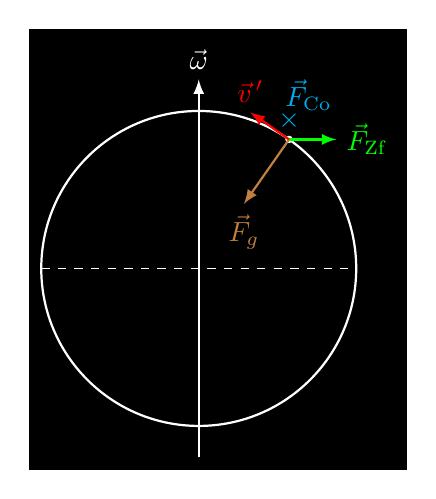
\begin{tikzpicture}[inverted,scale=2]
  \draw[dashed] (-1,0) -- (1,0);
  \draw[->,thick] (0,-1.2) -- (0,1.2) node[above] {$\vec{\omega}$};
  \draw[thick] (0,0) circle (1);
  \coordinate (r) at (55:1);
  \draw[fill=white] (r) circle (0.02);
  \draw[->,brown,thick] (r) -- (55:0.5) node[below] {$\F_g$};
  \draw[->,green,thick] (r) -- ++(0.3,0) node[right] {$\F_\text{Zf}$};
  \draw[->,red,thick]   (r) -- ++(55+90:0.3) node[above] {$\vec{v}^{\,\prime}$};
  \node[above,blue] at (r) {$\times$};
  \node[above,blue,xshift=0.7em,yshift=0.7em] at (r) {$\F_\text{Co}$};
\end{tikzpicture}
\end{document}
